\clearpage
\sect{5. Entrenamiento y rescate}

Juegas con Nick. Supera siete pruebas, vence al instructor y gradúate. Después entra en el edificio ocupado y rescata a los rehenes. Joe es tu rival en las pruebas que muestran a dos participantes.

\begin{enumerate}
\item \textbf{Carrera de obstáculos.} Gana velocidad y cruza la meta antes de que se agote el tiempo. Salta las vallas. Salta para agarrarte a las barras elevadas y sigue pulsando el botón de carrera para avanzar colgado.
\item \textbf{Galería de tiro I.} Apunta y acierta al menos \textbf{44} dianas. Las casillas se rellenan con los aciertos.
\item \textbf{Iron Man Race.} Atraviesa terreno difícil y agua antes de que se agote el tiempo. Dirige al corredor para esquivar obstáculos o vuelve atrás si te saltas un paso. La vista izquierda te sigue a ti y la derecha sigue a Joe.
\item \textbf{Galería de tiro II.} Muévete de lado a lado y acierta al menos \textbf{52} robots. Dispara a su paso cuando se acerquen.
\item \textbf{Pulso.} Pulsa rápido para ganar fuerza cuando empiece el combate. Si vences, consigues una bonificación. Pasas a la siguiente prueba con cualquiera de los dos resultados.
\item \textbf{Galería de tiro III.} Acierta al menos \textbf{32} dianas magenta. Si disparas a la silueta del instructor, los controles se bloquean hasta que aparece la siguiente tanda.
\item \textbf{Combate con el instructor.} Derríbalo antes de que se agote el tiempo. Vigila la energía de ambos y acércate cuando puedas acertar una patada.
\end{enumerate}

\begin{figure}[H]
\centering
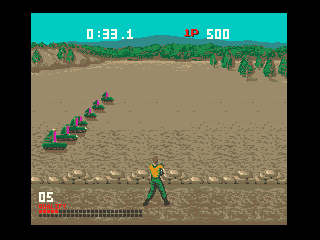
\includegraphics[width=.47\textwidth]{../img/robots.png}\hfill
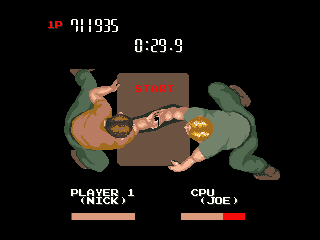
\includegraphics[width=.47\textwidth]{../img/arm-wrestling.png}
\caption{Galería de tiro II y comienzo del pulso.}
\end{figure}

\textbf{Misión final.} Tras graduarte, sigue el aviso y entra en el edificio. Salta sobre las cajas, usa las tuberías elevadas y esquiva los cuchillos y el fuego. Ábrete paso hasta el último rival y derrótalo para rescatar a los rehenes.

\clearpage
\sect{6. Cómo leer la pantalla}

\begin{figure}[H]
\centering
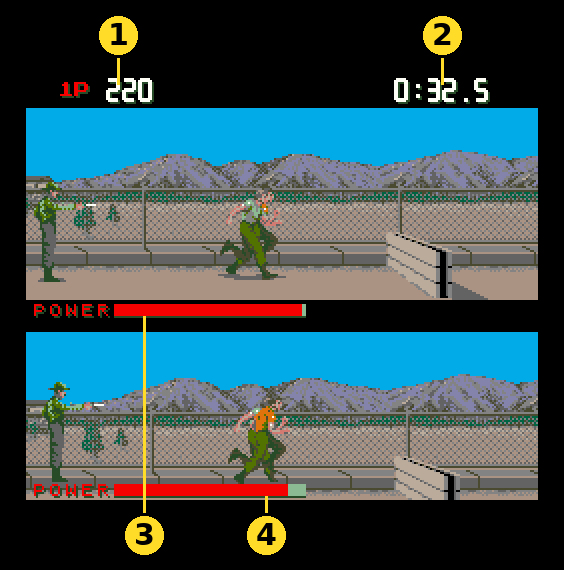
\includegraphics[width=.73\textwidth]{img/race-hud.png}
\caption{Carrera de obstáculos. La vista superior sigue a Nick y la inferior a Joe.}
\end{figure}

\begin{tabularx}{\textwidth}{@{}llX@{}}
\toprule
\textbf{\tNo} & \textbf{\tElement} & \textbf{\tTellsYou}\\
\midrule
1 & Marcador \texttt{1P} & Puntos acumulados en la partida.\\
2 & Reloj & Tiempo restante para completar la prueba.\\
3 & \texttt{POWER} superior & Potencia de Nick. Pulsa el botón de carrera para aumentarla.\\
4 & \texttt{POWER} inferior & Potencia de Joe, que está controlado por el MSX.\\
\bottomrule
\end{tabularx}

Las galerías muestran el reloj, la puntuación, la mira o la línea de tiro y las casillas de acierto. En el combate con el instructor, las barras de energía indican cuánto daño aguanta todavía cada luchador. Durante el último combate de la misión aparecen los indicadores de energía y puntuación.

\begin{figure}[H]
\centering
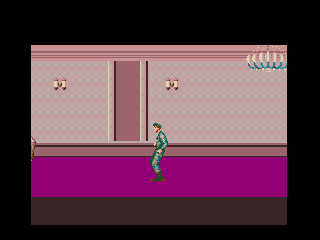
\includegraphics[width=.30\textwidth]{../img/mission.png}\hspace{1em}
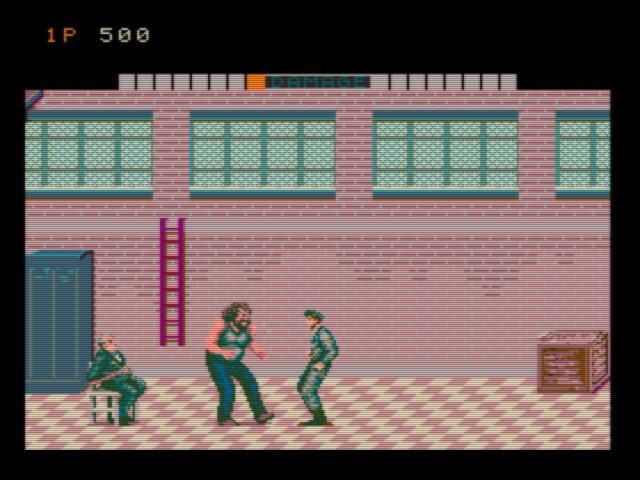
\includegraphics[width=.30\textwidth]{../img/boss.png}
\caption{De las primeras salas al combate final.}
\end{figure}

\clearpage
\sect{7. Reválida y puntuación}

\textbf{Dominadas.} Si fallas por poco en una carrera o galería, puedes tener una segunda oportunidad una sola vez por partida. Si el instructor te manda a la barra, espera a que Nick se agarre y pulsa repetidamente el botón de carrera hasta que el contador llegue a cero. Si acabas a tiempo, pasas a la siguiente prueba sin la bonificación de la que fallaste. El pulso no necesita reválida.

\begin{tabularx}{\textwidth}{@{}lX@{}}
\toprule
\textbf{Prueba} & \textbf{Puntuación}\\
\midrule
Carreras & Avanzar da puntos. En la carrera de obstáculos, saltar una valla sin trepar da 500 puntos extra.\\
Galerías I y III & Cada acierto da de 100 a 500 puntos, según su lugar en la tanda.\\
Galería II & Cada acierto da 100 puntos.\\
Pulso & Ganar da 4.000 puntos y añade tres segundos.\\
Instructor & Cada golpe da 500 puntos. El derribo del instructor da 100.000.\\
Misión final & Derrotar a enemigos y golpear al jefe da puntos. Vencer al jefe da 100.000.\\
\bottomrule
\end{tabularx}

Las bonificaciones se suman al marcador de la partida. Los segundos de bonificación que se muestran al completar una prueba se añaden a la siguiente que se indica.

\sect{8. Ranking}

Si tu puntuación entra entre las diez primeras, elige los caracteres con los cursores o el joystick. Arriba o derecha avanzan en la lista. Abajo o izquierda retroceden. Pulsa \key{ESPACIO} o el botón~1 para aceptar. Escribe tres caracteres o elige \texttt{END}. Las puntuaciones se conservan mientras el MSX siga encendido.

\begin{figure}[H]
\centering
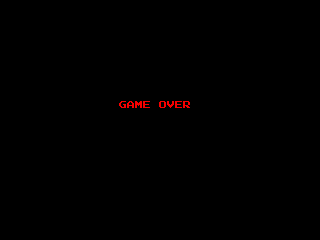
\includegraphics[width=.44\textwidth]{../img/game-over.png}\hfill
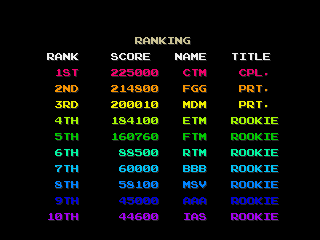
\includegraphics[width=.44\textwidth]{../img/ranking.png}
\caption{Fin de partida y ranking con puntuación, iniciales y grado.}
\end{figure}
